% !TEX root = ../PhD Thesis.tex

%\chapter{cTRAP: identification of candidate causal perturbations from differential gene expression data}
\chapter{cTRAP}
\label{chap:ctrap}

\begin{figure}[!b]
  \vspace*{-1cm}
  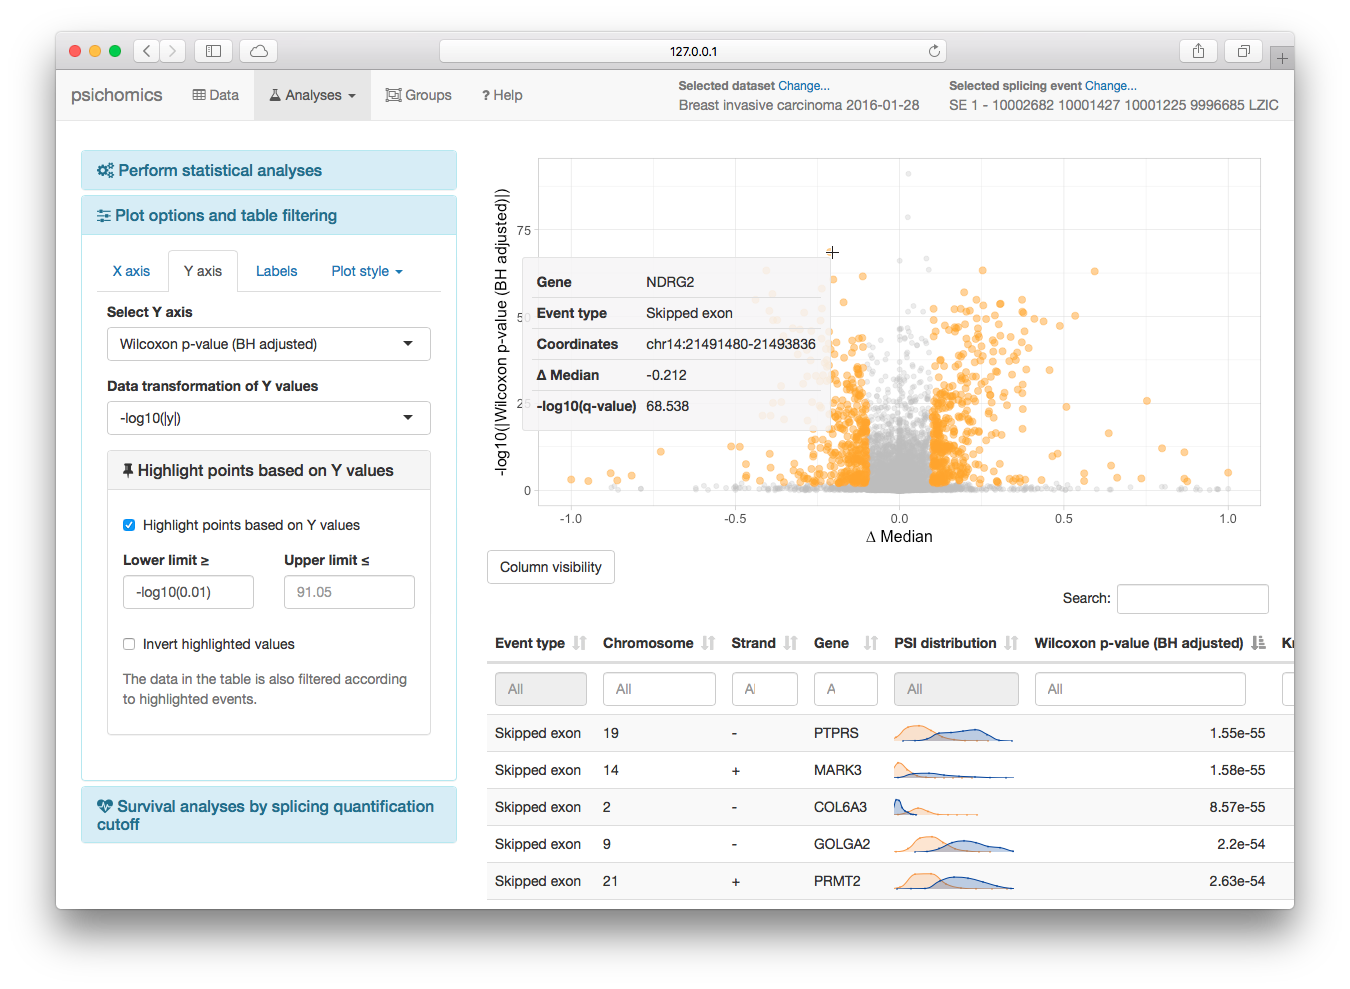
\includegraphics[width=0.96\textwidth]{images/cTRAP/screenshot}
  \centering
  \vspace*{-.5cm}
  \caption[cTRAP screenshot]{\textbf{cTRAP screenshot} (21 Dec 2021).}
  \label{fig:cTRAP-screenshot}
\end{figure}

Our lab had a brainstorm session during a stormy day in our 2017 Madeira retreat, where we discussed the unique propositions that the lab could provide to the scientific community.

One idea that emerged was to make it easier to identify putative causal perturbations by comparing a custom differential gene expression against the large-scale database of differential expression profiles from CMap \cite{subramanian:2017ul}, a repository of transcriptomic signatures for thousands of genetic (gene overexpression or knockout) and pharmacological perturbations in human cancer cell lines. This kind of analysis is available in CMap's web apps at \alink{clue.io} \cite{subramanian:2017ul}, but their results are difficult to integrate in downstream analyses, suffer from poor API documentation for programatic access and lack basic visualisation tools.

% clue.io does indeed allow for batch query: https://clue.io/connectopedia/batch_query_tutorial
% clue.io API's is not straightforward: https://clue.io/connectopedia/query_api_tutorial

To overcome those limitations, we developed cTRAP, an R package to compare user-provided differential gene expression profiles with the perturbations available from CMap, allowing to infer putative candidate molecular causes for the observed differences, as well as compounds that may promote or revert them.

After releasing the first version in Bioconductor, multiple features were added (\shortref{tab:cTRAP}). Inspired by the method used to compare gene expression changes against the CMap database, we also added a way to predict targeting drugs by using drug sensitivity datasets that featured gene expression for multiple genes in many cell lines. Moreover, we added a GSEA-based analysis of the enrichment of molecular descriptors for compounds from NCI60 and CMap. More recently, we developed a visual interface to host cTRAP online with support for user sessions and background tasks.

\begin{table}[!ht]
\parnotereset
\small
\caption[Major cTRAP milestones]{\textbf{Major cTRAP milestones.}}
\label{tab:cTRAP}
\begin{tabularx}{\textwidth}{ r r l }
\toprule
\textbf{Version} & \textbf{Release date} & \textbf{Main features} \\
\midrule
1.0.0  &  2 Nov 2018 & Compare differential expression profiles against CMap data\parnote{First Bioconductor release.} \\
1.4.0  & 12 Nov 2019 & Predict targeting drugs using NCI60, CTRP and GDSC data \\
       &             & Analyse drug set enrichment using molecular descriptors \\
1.8.0  & 30 Oct 2020 & Include graphical functions to load data and analyse results \\
1.10.0 & 20 May 2021 & Improve speed and memory usage when comparing data \\
1.12.0 & 28 Oct 2021 & Add web server support (optimised to run in ShinyProxy)\parnote{First version available online.} \\
\bottomrule
\end{tabularx}
\parnotes
\end{table}

The associated cTRAP manuscript (of which I am a co-first and co-corresponding author) is in preparation for submission to an international peer-reviewed scientific journal and shares some similarities with this chapter.

\section{Background}

The Connectivity Map (CMap) is a repository of transcriptomic signatures of thousands of genetic and pharmacological perturbations in human cancer cell lines \cite{subramanian:2017ul}. Comparing differential gene expression profiles with those from CMap allows to infer putative molecular causes for the observed differences, as well as compounds that may promote or revert those changes.

The CMap and LINCS Unified Environment (\alink{clue.io}) was developed as a collection of user-friendly tools for the manipulation of CMap data and their integration with user-provided data \cite{subramanian:2017ul}. However, \alink{clue.io} limits the maximum number of input genes for CMap queries, expresses results' significance in a non-standard significance score, is difficult to automate for downstream analyses and does not support using local computing resources. Furthermore, \alink{clue.io} does not currently integrate with drug sensitivity datasets, which could further assist in pinpointing compounds that selectively target cells.

We thus developed cTRAP, an R package and web app that identifies potentially causal molecular perturbations by seamlessly comparing full user-provided differential gene expression results with those available from CMap. cTRAP also supports comparisons with gene expression/drug sensitivity associations derived from the NCI-60 \cite{shoemaker:2006wi}, the Cancer Therapeutics Response Portal (CTRP) \cite{seashore-ludlow:2015ws} and the Genomics of Drug Sensitivity in Cancer (GDSC) \cite{yang:2012vk}, to identify compounds that could target the phenotypes associated with the user-provided differential expression profiles. In cTRAP, similarity is measured by gene set enrichment \cite{subramanian:2017ul,subramanian:2005wu} and correlation scores.

cTRAP can be installed using Bioconductor (\alink{bioconductor.org/packages/cTRAP}) or Docker (\dockerlink{nunoagostinho/ctrap}). The latest version of cTRAP is also available online at \alink{compbio.imm.medicina.ulisboa.pt/cTRAP}. The source code of cTRAP is available at \alink{github.com/nuno-agostinho/cTRAP}.

\section{Materials and methods}

From a vector of user-provided differential expression results (e.g. t-statistic values) with respective gene symbols, cTRAP can return a ranked list of similar CMap perturbations or predict targeting drugs. Moreover, cTRAP can also analyse the enrichment of drug sets in an ordered vector of compounds to identify common compound characteristics (\shortref{fig:ctrap-workflow}).

\begin{figure}[!ht]
  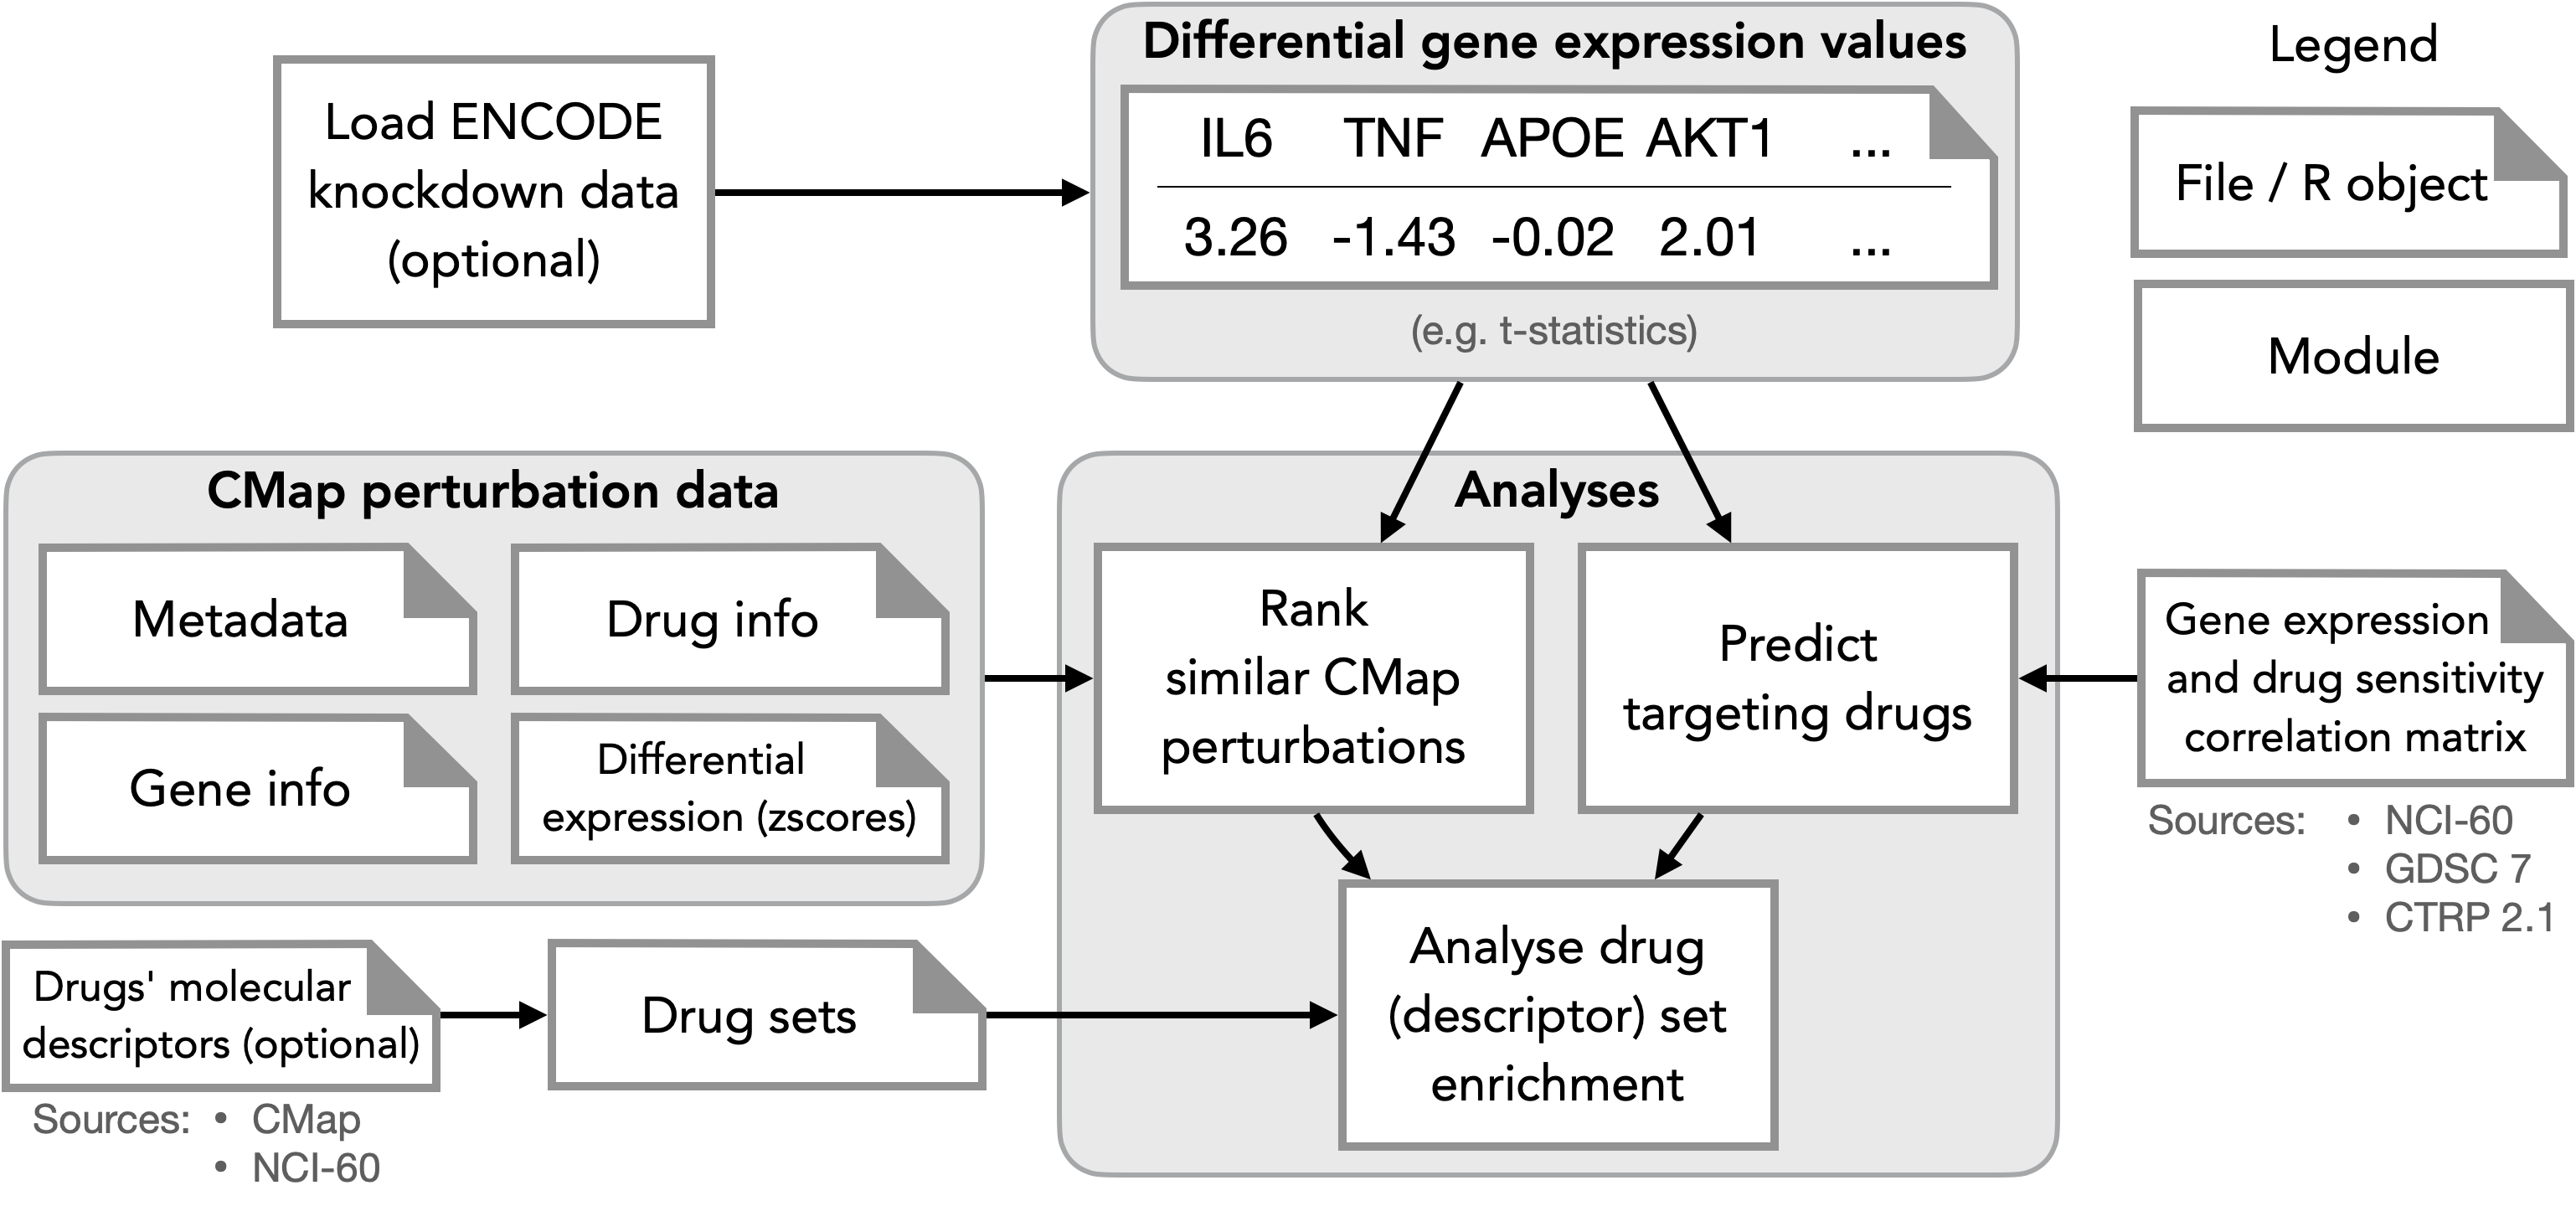
\includegraphics[width=1\textwidth]{images/ctrap/workflow}
  \centering
  \caption[cTRAP workflow]{\textbf{cTRAP workflow.} cTRAP allows to perform three analyses: \textbf{(1) rank similar CMap perturbations} by comparing user-provided differential gene expression values against CMap perturbation data, \textbf{(2) predict targeting drugs} by comparing user-provided differential gene expression values against correlation matrices of gene expression and drug sensitivity data and \textbf{(3) analyse drug (descriptor) set enrichment} using drug sets and the results from either the first or second analysis. CMap perturbation data, gene expression/drug sensitivity correlation matrices and drug molecular descriptors for drug sets can be automatically downloaded.}
  \label{fig:ctrap-workflow}
\end{figure}

\begin{figure}[!ht]
  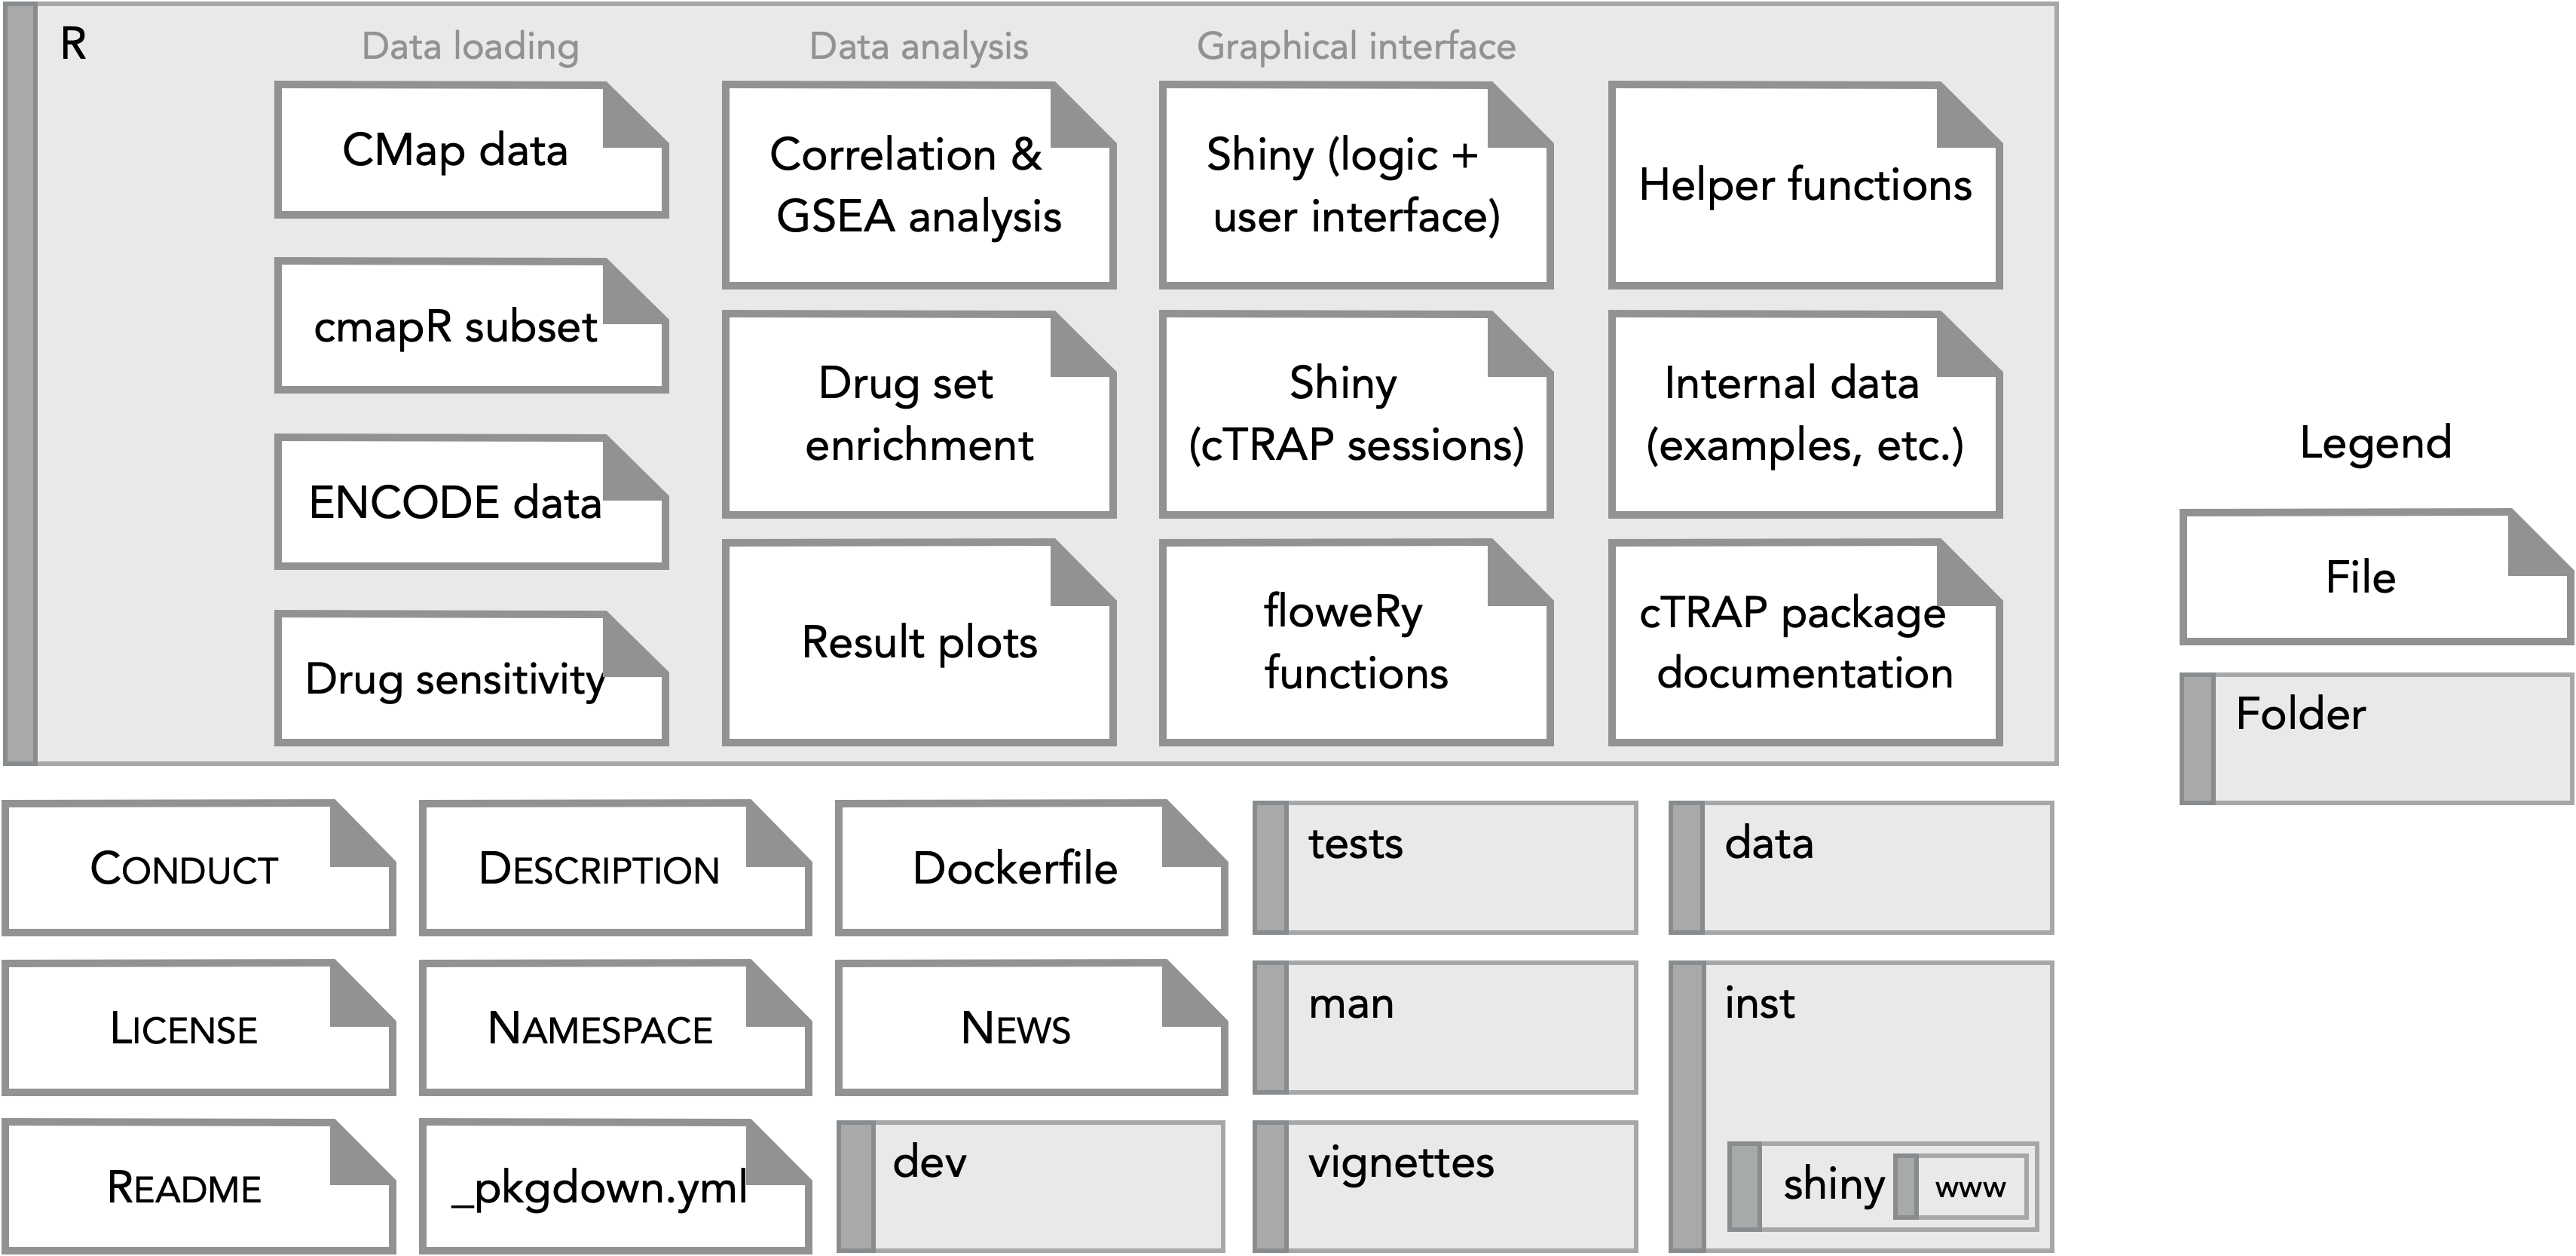
\includegraphics[width=1\textwidth]{images/ctrap/file-structure}
  \centering
  \caption[cTRAP file structure]{\textbf{Visual representation of cTRAP's file structure.} As usual in an R package, the \texttt{R} folder contains the scripts with cTRAP functions and data. \texttt{dev} is a custom folder that stores supporting scripts (e.g. test workflows and benchmarks); its contents are not included when building the R package.}
  \label{fig:ctrap-file-structure}
\end{figure}

\subsection{ENCODE knockdown data}

Using cTRAP, we can query and download ENCODE knockdown (and respective control) samples for multiple cell lines, filter low coverage counts from gene expression data, convert from ENSEMBL identifiers to gene symbol, and perform differential gene expression using \texttt{voom()}, \texttt{lmFit()} and \texttt{eBayes()} from the \texttt{limma} R package \cite{ritchie:2015tm}. First, \texttt{voom()} is used with the \emph{quantile} normalisation to transform count data to log\textsubscript{2} CPM (counts per million) and estimate the mean-variance relationship to compute weights used in linear modelling. Gene-wise linear models are then fitted using \texttt{lmFit()} between the knockdown and the control samples, followed by moderated t-tests and the calculation of log-odds of differential expression, using \texttt{eBayes()} for empirical Bayes moderation of standard errors.

cTRAP includes an example dataset (\texttt{diffExprStat}) with the differential gene expression results (t-statistic values) between the EIF4G1 knockdown in HepG2 versus control (\shortref{lst:diffExprStat}).

\begin{lstlisting}[caption=Code to obtain example dataset \texttt{diffExprStat}.,language=R,label={lst:diffExprStat}]
library(cTRAP)
ENCODEmetadata <- downloadENCODEknockdownMetadata(cellLine="HepG2",
                                                  gene="EIF4G1")
ENCODEsamples  <- loadENCODEsamples(ENCODEmetadata)[[1]]
counts         <- prepareENCODEgeneExpression(ENCODEsamples)

# Remove low coverage genes (>= 10 counts shared by >= 2 samples)
minReads   <- 10
minSamples <- 2
filter     <- rowSums(counts[ , -c(1, 2)] >= minReads) >= minSamples
counts     <- counts[filter, ]

# Convert ENSEMBL identifiers to gene symbols
counts$gene_id <- convertGeneIdentifiers(counts$gene_id)

# Perform differential gene expression (DGE) analysis
diffExpr <- performDifferentialExpression(counts)

# Get t-statistic values of DGE and respective gene names
diffExprStat <- diffExpr$t
names(diffExprStat) <- diffExpr$Gene_symbol
\end{lstlisting}

\subsection{Ranking of similar CMap perturbations}

CMap perturbations can be categorised into gene knockdown, gene over-expression and compounds. In cTRAP, available perturbation types and respective conditions can be enquired using the function \texttt{getCMapConditions()} that will download CMap perturbation metadata. Afterwards, the function \texttt{filterCMapMetadata()} allows to filter the metadata based on selected perturbations types, cell lines, dosages and time points, allowing to specifically load only the desired data in downstream analyses. This information is passed to \texttt{prepareCMapPerturbations()} to download (if file is not found) and process CMap differential expression profiles z-scores (GCTX file) and gene and compound information. Given that the GCTX file size is around 21GB, we recommend to download the file directly from GEO GSE92742’s Level 5 data link (\sloppy{\small{\url{ftp://ftp.ncbi.nlm.nih.gov/geo/series/GSE92nnn/GSE92742/suppl/GSE92742_Broad_LINCS_Level5_COMPZ.MODZ_n473647x12328.gctx.gz}}}).

\begin{figure}[!ht]
  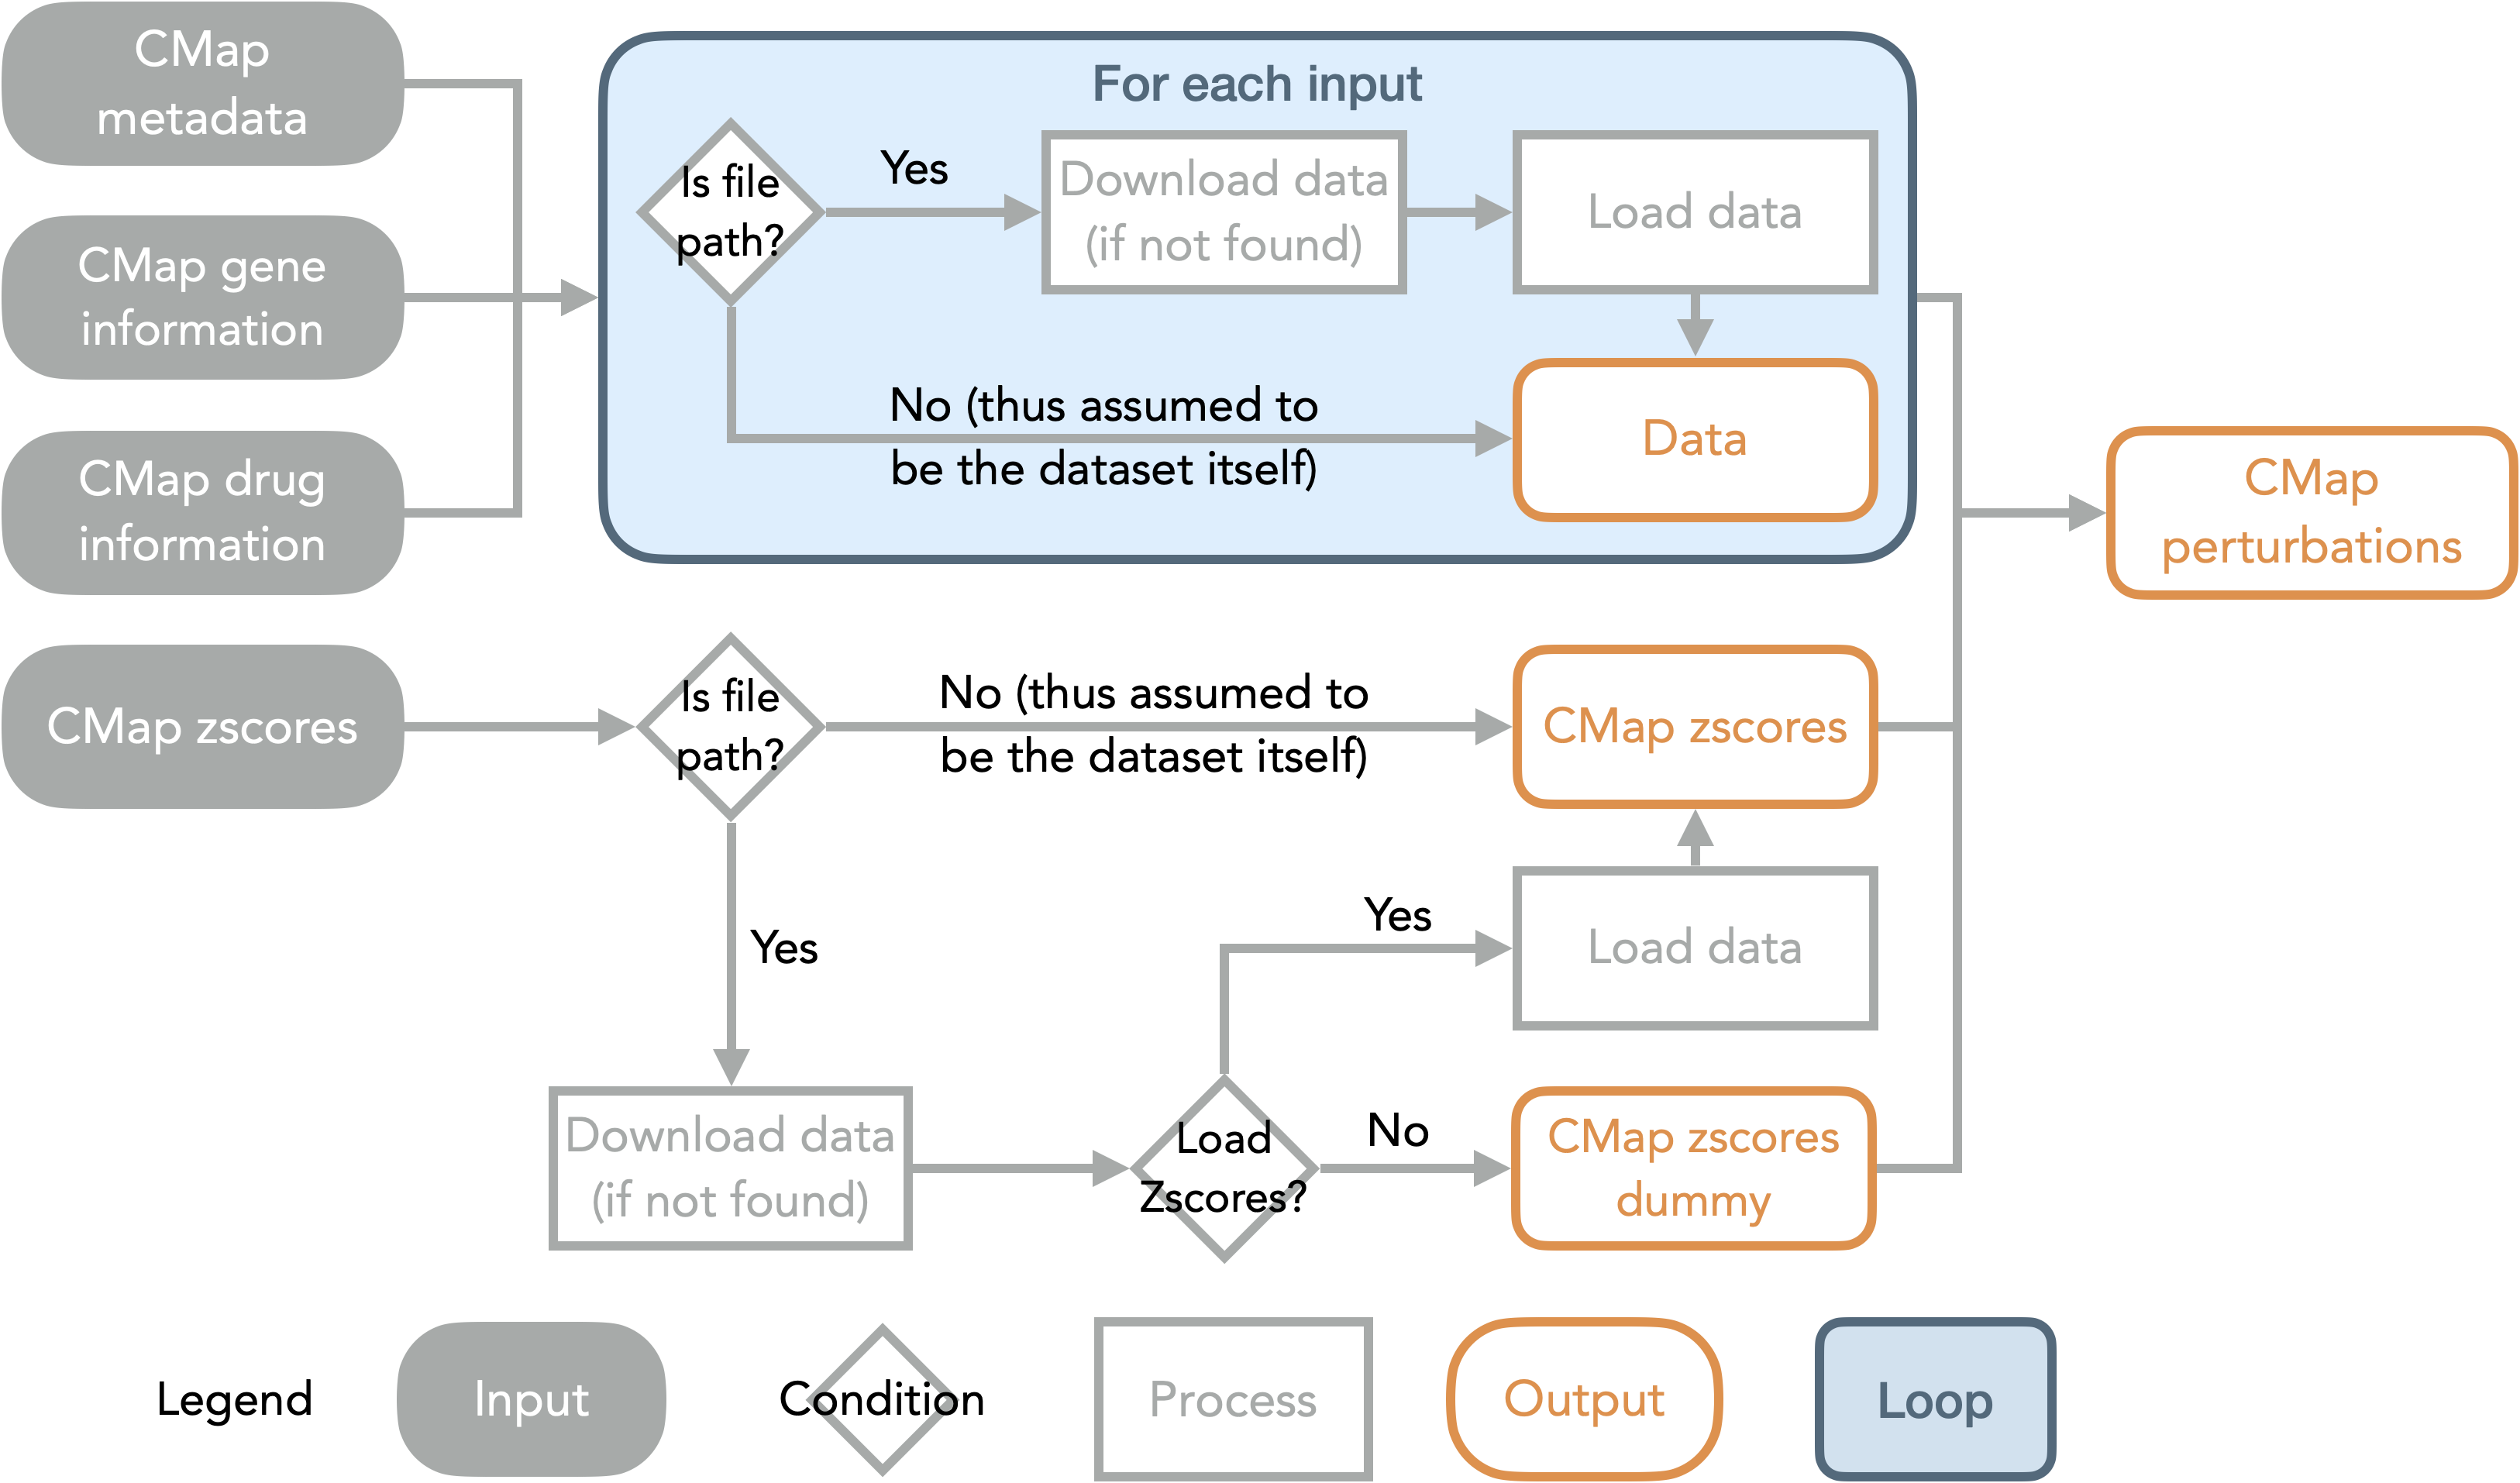
\includegraphics[width=.8\textwidth]{images/ctrap/cmap-perturbations}
  \centering
  \caption[Loading data from CMap perturbations]{\textbf{Loading data from CMap perturbations.} Input arguments support either the data itself (as data frames) or their respective file path. If the file path directs to a non-existing file,  data is first downloaded and then saved to the given file path. To avoid high memory usage, CMap perturbations' z-scores of differential expression profiles (CMap zscores) are not loaded into memory when a file path is given. Instead, only metadata are loaded into a \emph{dummy} object that can be subset as a normal R object for downstream analyses.}
  \label{fig:ctrap-cmap-perturbations}
\end{figure}

After comparing differential expression z-scores from select CMap perturbations against user-provided differential expression results, \texttt{rankSimilarPerturbations()} returns a table with ranked CMap perturbations and their respective correlation coefficients and GSEA scores. Lower ranks indicate perturbations whose differential expression profiles are more similar to the user-provided data, i.e. CMap perturbations that potentially mimic the user-provided transcriptomic changes, whereas higher ranks define perturbations that may revert those changes.

To rank CMap perturbations, cTRAP performs Spearman's and Pearson's correlations between the user-provided statistics for differential expression and values from CMap perturbations, and calculates a GSEA-based score (all three methods are run by default). For each method, the similarity scores are averaged across multiple cell lines for the same conditions (when available) and those averages are then used to rank CMap perturbations. By default, results for individual cell lines are provided for informative purposes (e.g. to check the heterogeneity of response across cell lines) but not used when ranking. The different ranking scores are combined via the rank product, ultimately used to sort the CMap perturbations. % rank product not properly explained

The GSEA-based score is calculated via the following steps:

\begin{enumerate}
	\item Sort genes from the user-provided differential expression statistics;
	\item Define the top 150 (by default) and bottom 150 (by default) genes as two sets
	\item For each CMap perturbation, sort genes by their differential expression z-scores and calculate the Weighted Connectivity Score (WTCS) \cite{subramanian:2017ul} based on the GSEA enrichment scores for the two sets.
\end{enumerate}

As an example, for a CMap perturbation with a similar differential expression profile to user’s input, we expect to find higher enrichment of the top gene set in the most up-regulated genes and higher enrichment of the bottom gene set in the most down-regulated genes.

\begin{figure}[!ht]
  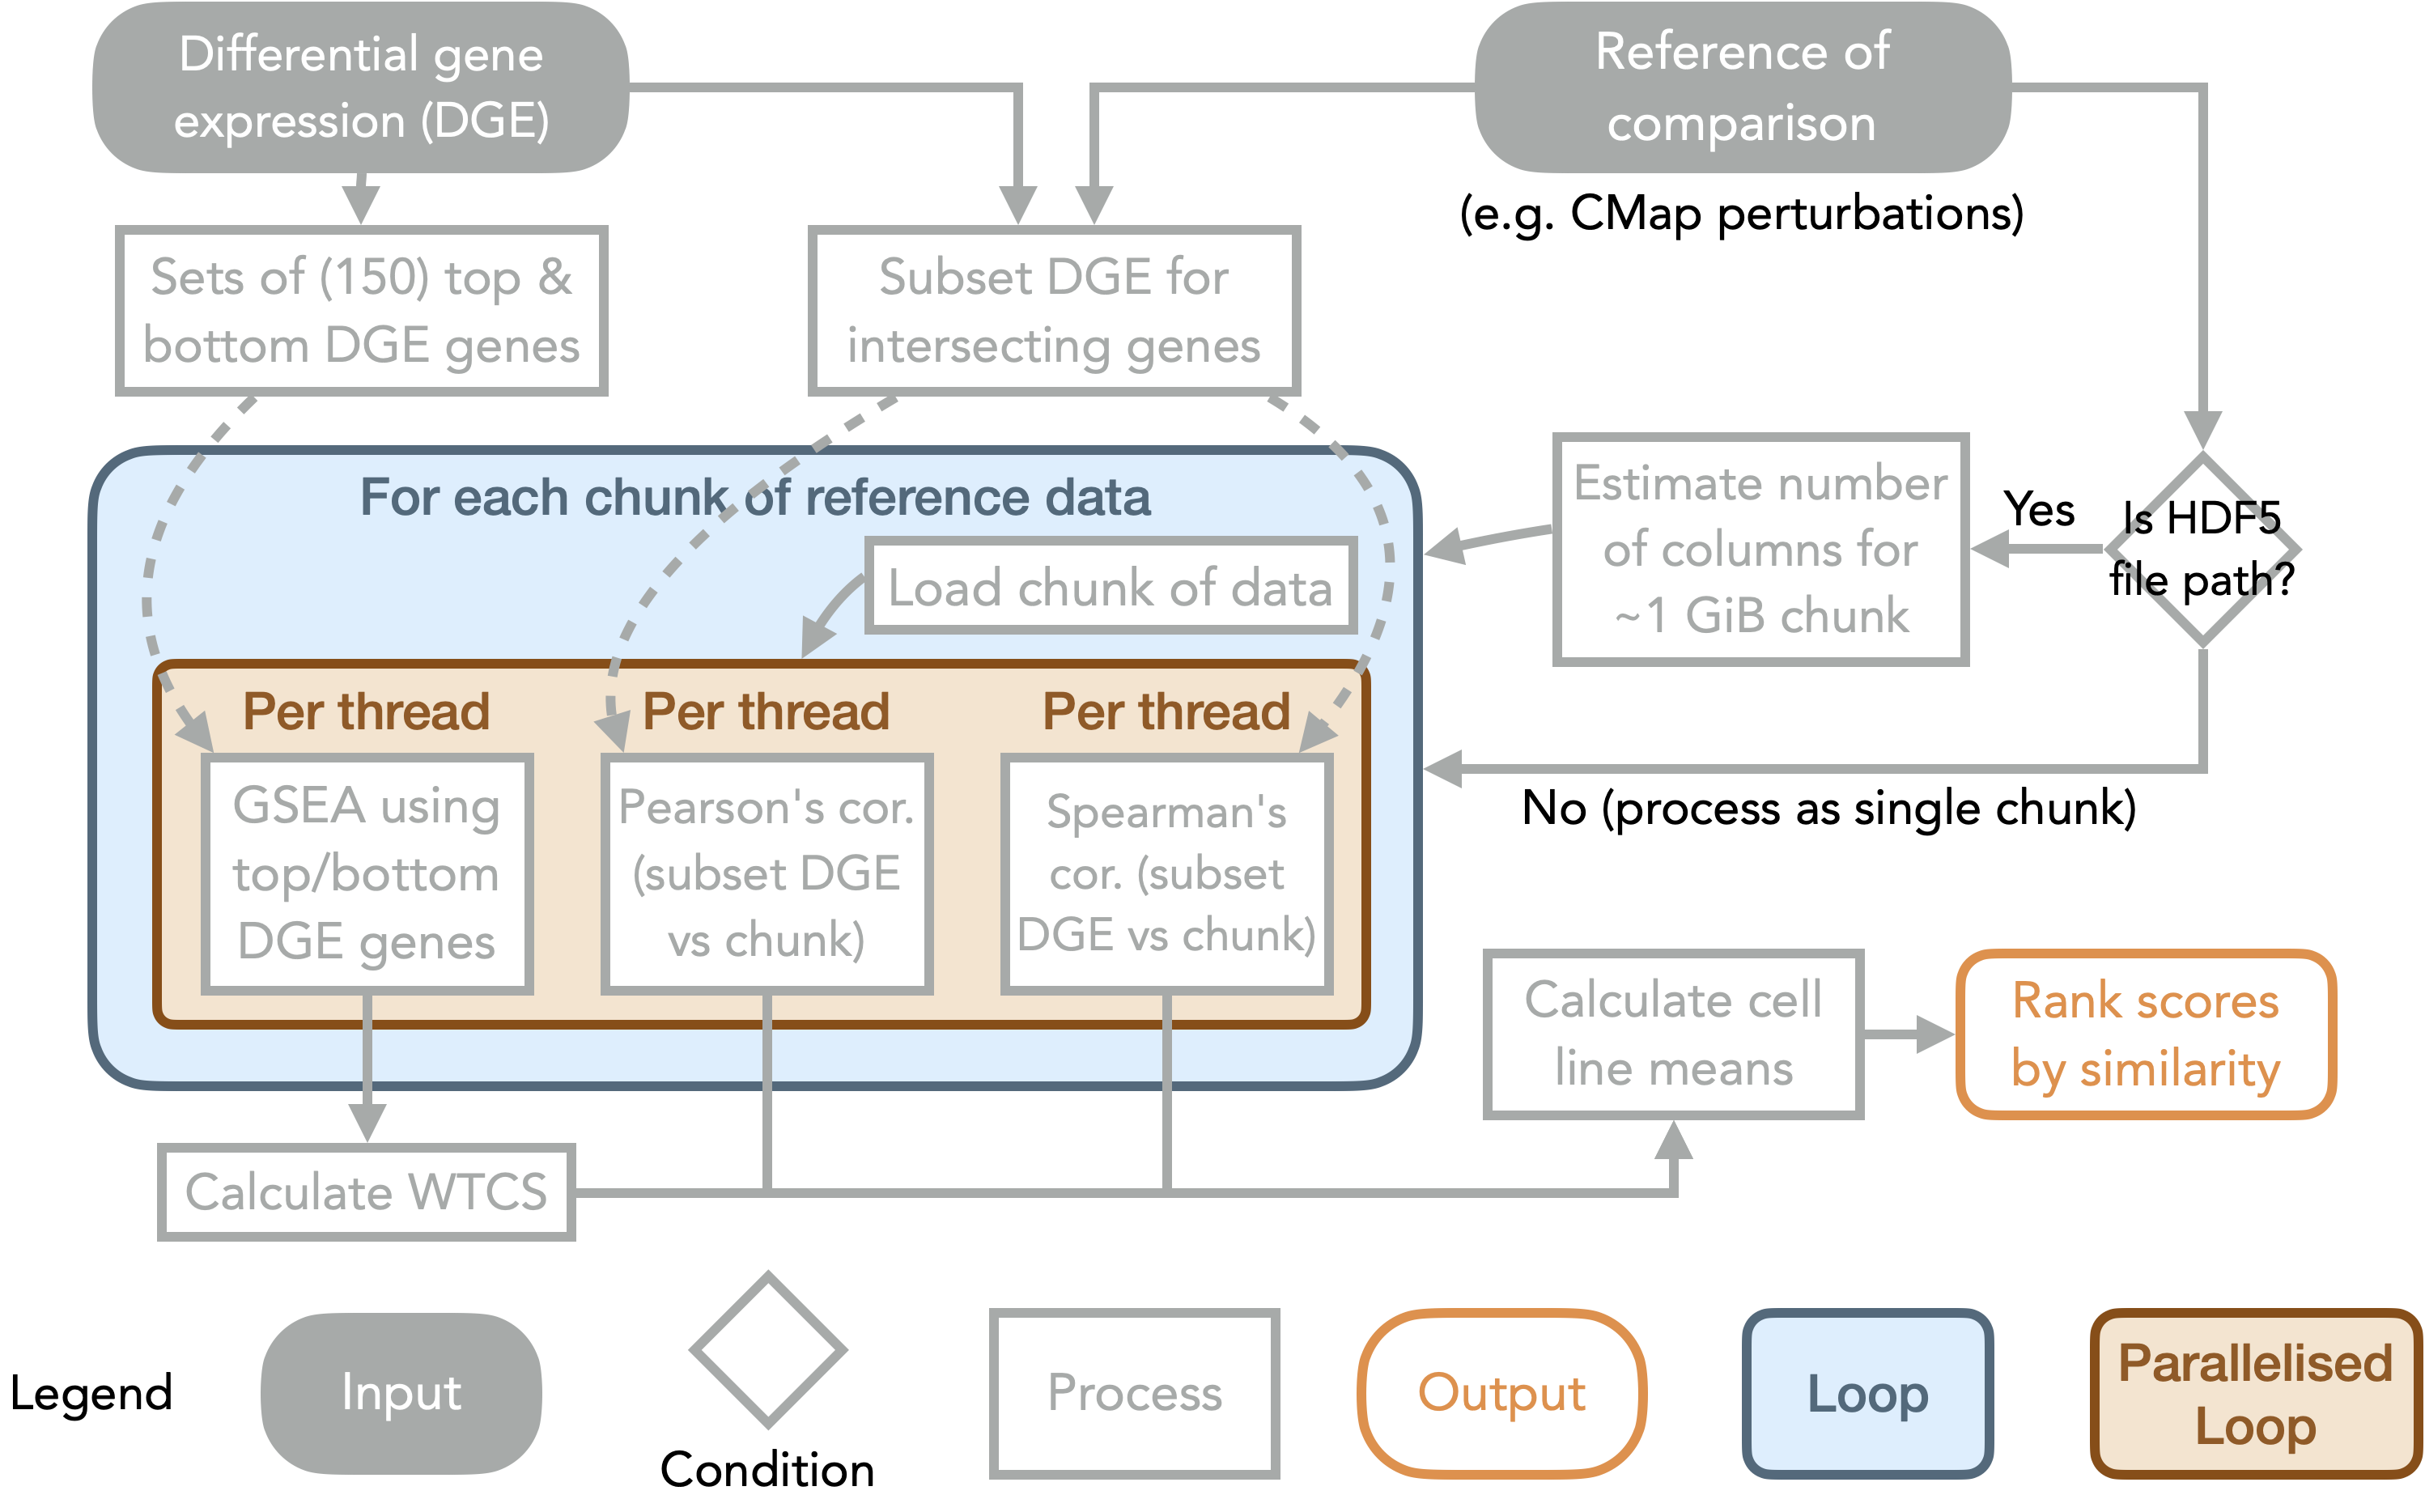
\includegraphics[width=.8\textwidth]{images/ctrap/analysis}
  \centering
  \caption[cTRAP similarity analysis]{\textbf{cTRAP similarity analysis.} User-provided differential gene expression is compared against a reference (e.g. differential expression z-scores of CMap perturbations) and ranked by similarity. If the reference of comparison is a HDF5 file path, the file is processed in 1GiB chunks to minimise peak memory usage. These analyses support multiple threads in Linux and macOS.}
  \label{fig:ctrap-analyses}
\end{figure}

To minimise peak RAM usage, \texttt{prepareCMapPerturbations()} downloads the GCTX file (technically, a customised HDF5 file) for the CMap’s perturbation differential expression z-scores (if not previously downloaded) and returns its path without loading the file content itself, creating a \emph{dummy} object that only stores its file path, perturbation names, gene symbols and other associated metadata (\shortref{fig:ctrap-cmap-perturbations}). Based on the file path of this \emph{dummy} object (that can be subset like a normal R object), \texttt{rankSimilarPerturbations()} loads a $\le$ 1 GiB chunk\footnote{The default 1 GiB ($1024^3$ bytes) allows loading chunks of around 10000 columns and 14000 rows ($10000 \times 14000 \times 8 \textrm{ bytes} / 1024^3 = 1.04 \textrm{ GiB}$). CMap's GCTX file has around 14000 rows (genes).}, compares its differential expression z-score values against user-provided data and repeats the analysis for the next chunk (\shortref{fig:ctrap-analyses}). For each chunk, multithreaded support for Linux and macOS can be enabled for each comparison method via the \texttt{mclapply()}\footnote{\texttt{mclapply()} allows parallel computing via forking where child processes are spawned from a parent process and share their memory. Forking is unavailable in Windows and current multithreaded alternatives need multiple copies of the same data chunk for each thread, requiring multiple slow copy operations for 1GiB chunks that slowed down the runtime of the analyses when prototyping.} function from R package \texttt{parallel} that can enabled by setting the number of threads to 2 or higher.

The ranked list from \texttt{rankSimilarPerturbations()} can be plotted using \texttt{plot()}, showing a list of all results ordered by a given score or either a scatterplot or GSEA plot for a predicted targeting drug.

\subsection{Prediction of targeting drugs}

Gene expression and drug activity data across multiple cell lines are available from NCI-60 \cite{shoemaker:2006wi}, Cancer Therapeutics Response Portal (CTRP) 2.1 \cite{seashore-ludlow:2015ws} and Genomics of Drug Sensitivity in Cancer (GDSC) 7 \cite{yang:2012vk}. For each source, the internal function \texttt{prepareExpressionDrugSensitivityAssociation()} performs the following steps:

\begin{enumerate}
	\item Download all the necessary data depending on given source;
	\item Perform Spearman’s correlation (by default) between the expression of each gene against the sensitivity of intersecting cell lines to each drug;
	\item Generate a matrix with the correlation coefficients per gene and drug; and
	\item Prepare metadata for downstream analyses, including gene, compound and cell line information from each source.
\end{enumerate}

A higher correlation coefficient for a given gene and drug suggests a gene whose higher expression is associated with higher drug sensitivity across multiple cell lines. As this process can take multiple hours to finish for all sources, the resulting objects were stored online for each aforementioned source and can be listed with \texttt{listExpressionDrugSensitivityAssociation()} and downloaded and loaded into R using \texttt{loadExpressionDrugSensitivityAssociation()}.

To identify compounds that could target the phenotype associated with specific differential expression profiles, we use \texttt{predictTargetingDrugs()} with those profiles and a correlation matrix of gene expression and drug sensitivity as input. The correlation coefficients between gene expression and drug sensitivity for each drug are compared against user-provided differential expression results by Spearman’s and Pearson’s correlation and GSEA-based scores (as performed when ranking CMap perturbations, results from comparison methods are ranked and then those rankings are finally used to calculate the rank product’s rank). \texttt{predictTargetingDrugs()} returns a table with ranked predicted targeting drugs and their respective correlation coefficients and GSEA scores (\shortref{fig:ctrap-analyses}). A lower rank comprise drugs that may target phenotypes similar to the user-provided differential expression profile.

The resulting object can be plotted with \texttt{plot()}, showing a list of all results ordered by a given score or either a scatterplot or GSEA plot for a predicted targeting drug.

The function \texttt{plotTargetingDrugsVSsimilarPerturbations()} compares the results from predicted targeting drugs and CMap perturbations that may mimic or revert the observed phenotype. For the available compound identifiers in the metadata pertaining from the different datasets (e.g. compound name, Broad ID, PubChem CID and SMILES), the function will automatically select the identifiers with higher number of matching values between the two datasets, unless the identifiers are explicitly defined by the user. A scatterplot is then returned using, by default, the rank product’s rank of targeting drugs in one axis and the rank product’s rank of similar perturbations in the other.

\subsection{Drug descriptor set enrichment analysis}

Juan Carlos, a former member of the lab, computed drug descriptors (e.g. molecular weight and number of aromatic rings) for compounds from CMap and NCI-60 based on their three-dimensional (3D) and two-dimensional (2D) characteristics. These descriptors were uploaded to \alink{compbio.imm.medicina.ulisboa.pt/public/cTRAP/} and the resulting files can be automatically downloaded and processed to R using \texttt{loadDrugDescriptors()}.

\texttt{prepareDrugSets()} allows to create sets of descriptors. By default, the function creates a maximum of 15 sets per drug descriptor. For each alphanumeric descriptor, one set is created per unique value of that descriptor. Alphanumeric descriptors containing more than 15 unique values (by default) will be discarded. For numerical descriptors, \texttt{prepareDrugSets()} internally uses the \texttt{binr::bins()} function to create evenly-distributed bins of drug descriptors, where each set contains a minimum number of points equal to the number of non-missing values divided by the number of maximum sets (15 by default) divided by a constant (5 by default).

The function \texttt{analyseDrugSetEnrichment()} analyses the enrichment of the created drug descriptor sets in a named numeric vector or an object returned from \texttt{rankSimilarPerturbations()} – only if run against CMap compound perturbations – or \texttt{predictTargetingDrugs()}. The GSEA-based enrichment analysis is internally performed using \texttt{fgsea::fgsea()}.

The resulting object can be plotted with \texttt{plot()}, showing a list of all results ordered by a given score or either a scatterplot or GSEA plot for a predicted targeting drug.

\subsection{Time and memory benchmarking}

We measured elapsed time using R’s \texttt{Sys.time()} immediately before and after ranking similar CMap perturbations, predicting targeting drugs (using NCI60 expression and drug sensitivity association, the most time-consuming option) and performing drug set enrichment analysis using cTRAP 1.8.1 (296f9b21). As input, we used the t-statistics for the differential expression between EIF4G1 knockdown versus control based on ENCODE gene expression data from cell line HepG2 (the \texttt{diffExprStat} object in the cTRAP package).

We measured the heap memory usage of cTRAP 1.8.1 (296f9b21) across time by running R 4.0.3 in debug mode with the heaptrack 1.0.0 profiler. heaptrack tracks and logs all calls to the core memory allocation functions via \verb|LD_PRELOAD| and respective backtraces. For R to work properly with heaptrack, the file \path{/usr/bin/R} was edited -- all lines of the last \emph{if} statement were commented out, except for:

\begin{lstlisting}[language=bash,numbers=none]
exec ${debugger} ${debugger_args} "${R_binary}" ${args} "${@}"
\end{lstlisting}

Afterwards, we benchmarked R scripts running cTRAP with:

\begin{lstlisting}[language=bash,numbers=none]
R -d heaptrack -f ${cTRAP_Rscript} --args ${cTRAP_Rscript_args}
\end{lstlisting}

All benchmarks were run in a workstation running Ubuntu 18.04.5 LTS with 768 GB of RAM memory and 72 cores (Intel Xeon Gold 6254 CPU @ 3.10GHz). The benchmarked cTRAP scripts are publicly available in cTRAP's GitHub repository: \alink{github.com/nuno-agostinho/cTRAP/tree/master/dev/benchmark}

\subsection{Continuous integration}

Similarly to psichomics (\fullref{subsec:psichomics-ci}), cTRAP uses GitHub Actions to:
\begin{itemize}
	\item Update Docker images in Docker Hub (\dockerlink{nunoagostinho/ctrap}) and GitHub (\alink{github.com/nuno-agostinho/cTRAP});
	\item Update website documentation using \texttt{roxygen} \cite{wickham:2021wt} and \texttt{pkgdown} \cite{wickham:2021wj};
	\item Build and test cTRAP in Windows, macOS and Linux.
\end{itemize}

\section{Results}

\subsection{Case study}

\subsection{Time and memory optimisation}

Show benchmarks.

\subsection{Graphical interface}

One of the most recent features is the support for visual interfaces that interactively perform most cTRAP features via the web browser. The graphical interface was modularly built and exposed via 5 functions that work harmoniously with R code:

\begin{itemize}
	\item \texttt{launchDiffExprLoader()} to load differential expression data. Returns a differential expression object that can be used in cTRAP analyses.
	\item \texttt{launchCMapDataLoader()} to explore and load CMap data by type of perturbation, cell types, time points and dosages. Returns filtered CMap data based on the user's selection.
	\item \texttt{launchMetadataViewer()} to check metadata of given cTRAP objects.
	\item \texttt{launchResultPlotter()} to view and plot cTRAP results given as input.
	\item \texttt{launchDrugSetEnrichmentAnalyser()} to analyse drug set enrichment and visualize respective results.
\end{itemize}

Like usual R functions, these graphical interfaces functions accept input and may return output. Thus, they can be intertwined with R code, allowing to easily reproduce cTRAP analyses (\shortref{lst:cTRAP-graphical}).

\begin{lstlisting}[caption=Calling CTRAP's graphical interface functions in an R script.,label={lst:cTRAP-graphical},language=R,morekeywords={include, launchDiffExprLoader},keywordstyle=\bfseries]
# Launch differential expression loading interface to select knockdown
# data from ENCODE (pre-filtered for HepG2 cell line and EIF4G1 gene)
diffExpr <- launchDiffExprLoader(cellLine="HepG2", gene="EIF4G1")

# After filter selection, launchDiffExprLoader() does the following:
# 1. Download ENCODE's HepG2 data for EIF4G1 knockdown and controls
# 2. Perform DGE between EIF4G1 knockdown vs. control
# 3. Return resulting t-statistics by gene

# Load CMap knockdown data in HepG2
cmapKD <- launchCMapDataLoader(
    cellLine="HepG2",
    perturbationType="Consensus signature from shRNAs targeting the same gene")
# Load CMap compound data in HepG2
cmapCompounds <- launchCMapDataLoader(cellLine="HepG2",
                                      perturbationType="Compound")
# Load all CMap data in HepG2
cmapPerts <- launchCMapDataLoader(cellLine="HepG2")

# View metadata of all resulting CMap data objects
launchMetadataViewer(cmapKD, cmapCompounds, cmapPerts)

# Rank similar perturbations -----------------------------------------
compareKD        <- rankSimilarPerturbations(diffExpr, cmapKD)
compareCompounds <- rankSimilarPerturbations(diffExpr, cmapCompounds)
comparePerts     <- rankSimilarPerturbations(diffExpr, cmapPerts)

launchResultPlotter(compareCompounds, compareKD, comparePerts)

# Predict targeting drugs --------------------------------------------
listExpressionDrugSensitivityAssociation()
assocMatrix <- listExpressionDrugSensitivityAssociation()[[1]]
assoc       <- loadExpressionDrugSensitivityAssociation(assocMatrix)
predicted   <- predictTargetingDrugs(diffExpr, assoc)
launchResultPlotter(predicted)

# Plot targeting drugs vs similar perturbations ----------------------
launchResultPlotter(predicted, compareCompounds)

# Analyse drug set enrichment ----------------------------------------
descriptors <- loadDrugDescriptors("NCI60", "3D")
drugSets    <- prepareDrugSets(descriptors)

launchDrugSetEnrichmentAnalyser(drugSets, compareCompounds)
launchDrugSetEnrichmentAnalyser(drugSets, predicted)
\end{lstlisting}

In order to increase its usefulness to the scientific community, cTRAP is available online\footnote{More information in \fullref{chap:app-server}} with a comprehensive interface that provides most aforementioned features in a single app via a sixth function: \texttt{cTRAP()}. A clear question arrived with such a strategy: how to deal with long-running tasks? The way R/Shiny is built, an entire cTRAP session would be consuming useful resources during the cTRAP analyses, but this would not properly scale for multiple users using heavy memory resources simultaneously. To avoid this, long-running tasks are put in a queue depending on available resources and performed in the background. But this also meant that the users would need get their results back once finished calculating. And thus the idea of user sessions was born.

\subsubsection{User sessions}
\label{sec:ctrap-web}

\begin{wrapfigure}{r}{.4\textwidth}
  \vspace{-2\intextsep}
  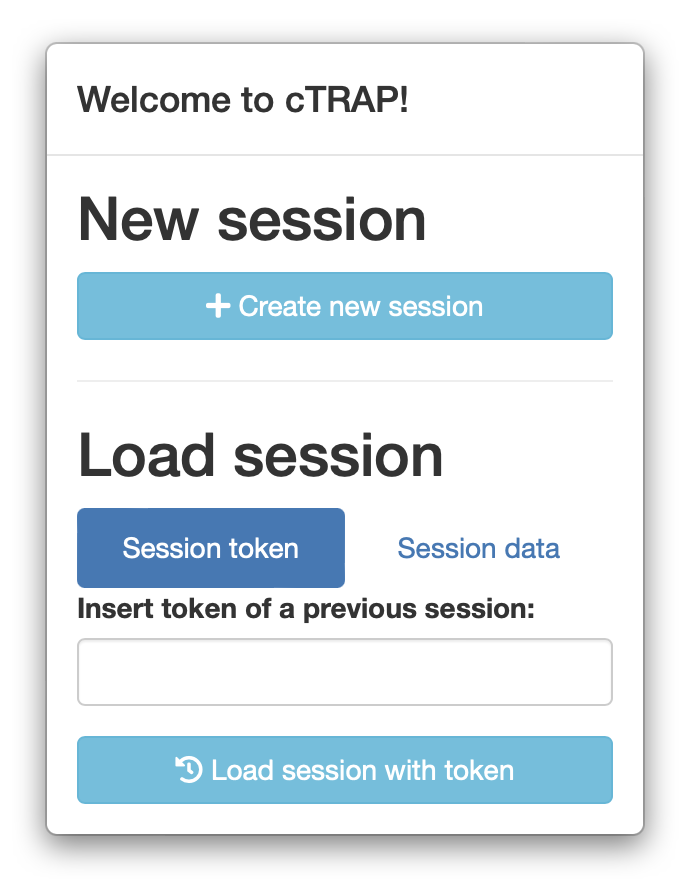
\includegraphics[width=\linewidth]{images/ctrap/welcome}
  \caption[Welcome screen modal]{\textbf{Welcome modal.}}
  \vspace{-1\intextsep}
  \label{fig:ctrap-welcome}
\end{wrapfigure}

When visiting cTRAP, a user is greeted with a welcome screen that allows to create a new session or restore a previous one (\autoref{fig:ctrap-welcome}). If the user clicks to create a new session, a random alphanumeric string (token) is created. The token will be the name of the folder storing user data and cTRAP ensures that the token is unique and no other folder is currently using it (\autoref{fig:user-session}).

% TODO: mention other files in common across cTRAP?
If the user loads data to their session, a new folder is named after the session token (\autoref{fig:user-session}). All updates to the session data are immediately saved to the session folder. To avoid downloading commonly-used files across sessions (e.g. the big 21GB CMap perturbations z-scores file), those files can be made available in a folder accessible to all sessions, thus skipping the step of downloading and preparing the data.\footnote{This is how cTRAP is configured in our web server.}

While using cTRAP, the user can create a new session and load a previous session via a token or a RDS file at any time. When using the token, cTRAP loads the contents of the folder named after the token – if no such folder exists, it will warn the user (\autoref{fig:user-session}). In case the user uploads a RDS file, cTRAP will create a new session and load the contents of the RDS file as the data session (\autoref{fig:user-session}). Using an RDS file ensures the user can open the data in an R session in their local computer given that this RDS file simply contains a list of all the datasets available in the session or even use this object in a local version of cTRAP. Moreover, as sessions start to accumulate in our server, they may be removed from the system and thus may become inaccessible\footnote{We have considered implementing a 14-day expiration period for user sessions. This is not currently in place.}.

\begin{figure}[!ht]
  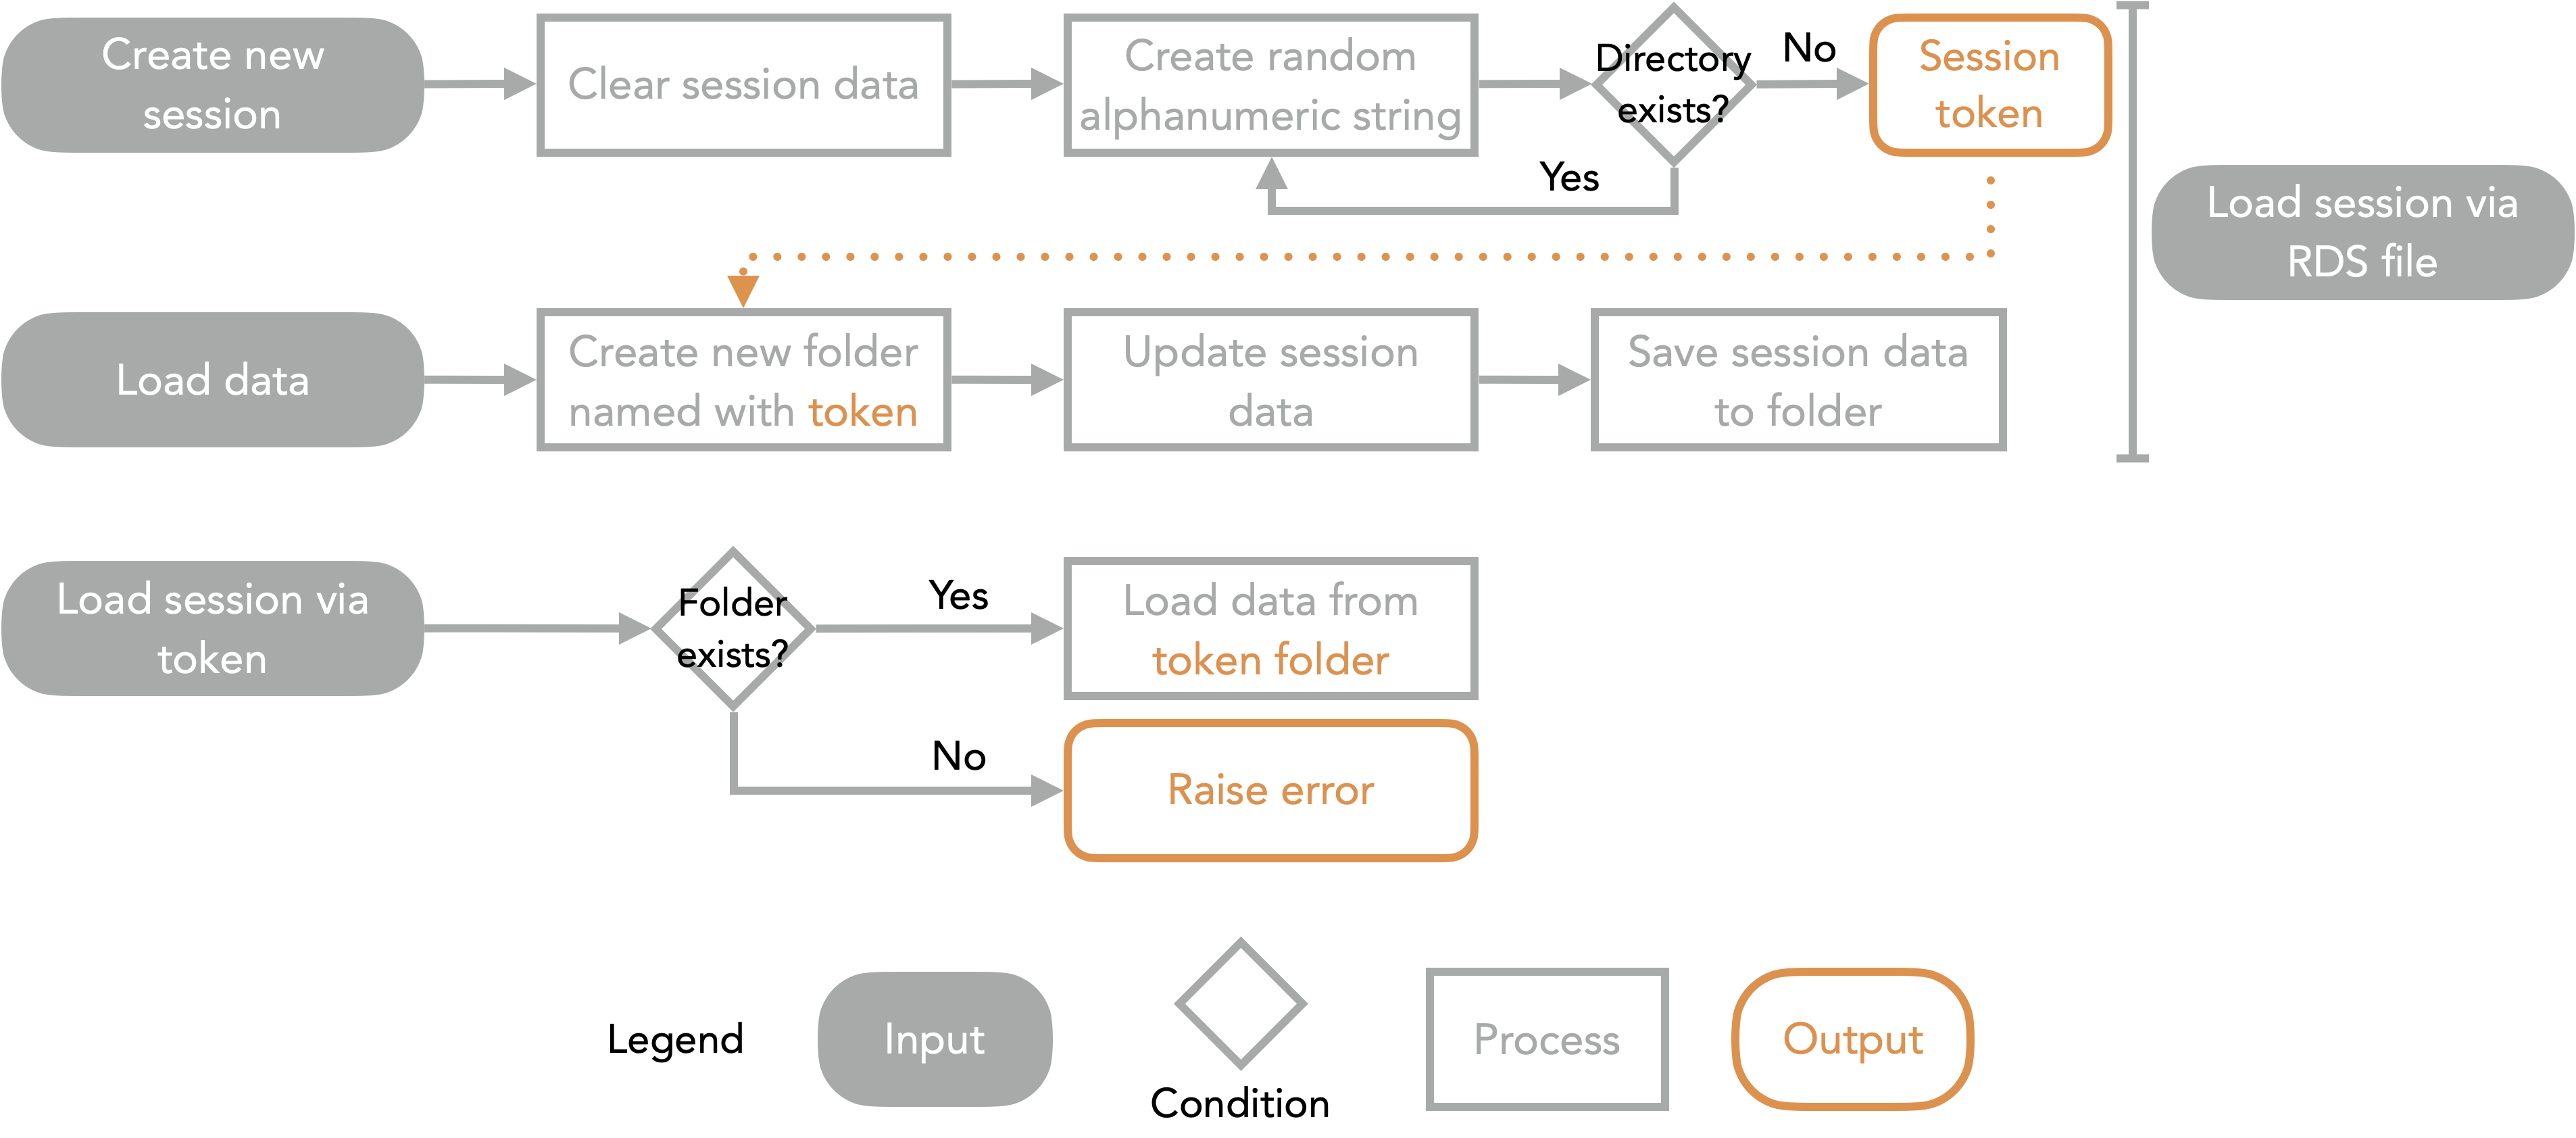
\includegraphics[width=\textwidth]{images/ctrap/user-session}
  \centering
  \caption[User session workflow]{\textbf{User session workflow.} cTRAP allows to create new sessions or load a previous one via a given token or RDS file.}
  \label{fig:user-session}
\end{figure}

\subsubsection{Background tasks}

As usual in an R/Shiny app, cTRAP runs tasks in the same R process as the app itself. The user has to wait for the long-running tasks to finish before being able to interact again with the app. Critically, if cTRAP is shut down, all running processes will stop. These issues can be overcomed by running tasks in the background using:

\begin{itemize}
	\item Celery, a task queue manager written in Python; and
	\item Flower, a monitoring app that provides an HTTP API for Celery.
\end{itemize}

In order to run cTRAP analyses via Celery, both cTRAP and Celery must be installed in the same system. Celery requires a \texttt{tasks.py} file with its tasks defined. For cTRAP, one of these tasks must be set up to run R commands via Python's \texttt{subprocess} module to spawn new processes and using the \texttt{Rscript} front-end (\shortref{lst:tasks.py}).

\begin{lstlisting}[language=python,caption=An example \texttt{tasks.py} file to run R commands or Rscript files via Celery.,label={lst:tasks.py},morekeywords={import},keywordstyle=\bfseries]{tasks.py}
import os, time
from datetime import datetime
from subprocess import run, PIPE

# Celery configuration
from celery import Celery
os.environ.setdefault('C_FORCE_ROOT', 'true')
app = Celery(
    "tasks",
    broker=os.environ.get('CELERY_BROKER_URL', 'redis://redis'),
    backend=os.environ.get('CELERY_RESULT_BACKEND', 'redis://redis'))
app.conf.CELERY_WORKER_SEND_TASK_EVENTS = True

# Runs R command and returns output
#   - Use cat(), e.g. 'cat(2+2)', to capture output as a job result
#   - Errors will result in a task state of FAILURE
def execR(cmd):
    return run(cmd, check=True, stdout=PIPE, text=True).stdout

# Run a given R expression as a Celery job
@app.task
def R(cmd): return execR(["Rscript", "-e", cmd])

# Run a given Rscript file as a Celery job
@app.task
def Rscript(cmd): return execR(["Rscript", cmd])

if __name__ == "__main__": app.start()
\end{lstlisting}

Celery can receive its jobs via HTTP methods from Flower, facilitating the communication between cTRAP and Celery. To assist using Flower's HTTP API, I created the R package floweRy (\alink{github.com/nuno-agostinho/floweRy}) to simplify sending jobs to Celery using R, as briefly demonstrated in \shortref{lst:httr} and \shortref{lst:floweRy}.

\noindent\begin{minipage}{.48\textwidth}
\begin{lstlisting}[caption=Using plain \texttt{httr}.,language=R,label={lst:httr}]{httr}
library(httr)
flower <- function(...) paste0(
    "http://localhost:5555", ...)
# Run R command '3 + 4' in Celery
POST(flower("/api/task/apply/tasks.R")), body="3 + 4", encode="json")
# Get status of all Celery tasks
GET(flower("/api/tasks"))
\end{lstlisting}
\end{minipage}\hfill
\begin{minipage}{.48\textwidth}
\begin{lstlisting}[caption=Using \texttt{floweRy}.,language=R,label={lst:floweRy}]{floweRy}
library(floweRy)
options(flowerURL=
    "http://localhost:5555")
# Run R command '3 + 4' in Celery
taskApply("tasks.R", "3 + 4")


# Get status of all Celery tasks
taskList()
\end{lstlisting}
\end{minipage}

cTRAP currently supports ranking similar CMap perturbation and predicting targeting drugs as background processes. The user can monitor the status of their background tasks in cTRAP. When the background processes finish, Celery output files are saved into the session folder. The data is then automatically loaded and the user is informed of such via a notification in cTRAP (\shortref{fig:ctrap-celery}). If the user has closed the session, this process will occur when the cTRAP session is loaded via its token.

\begin{figure}[!ht]
  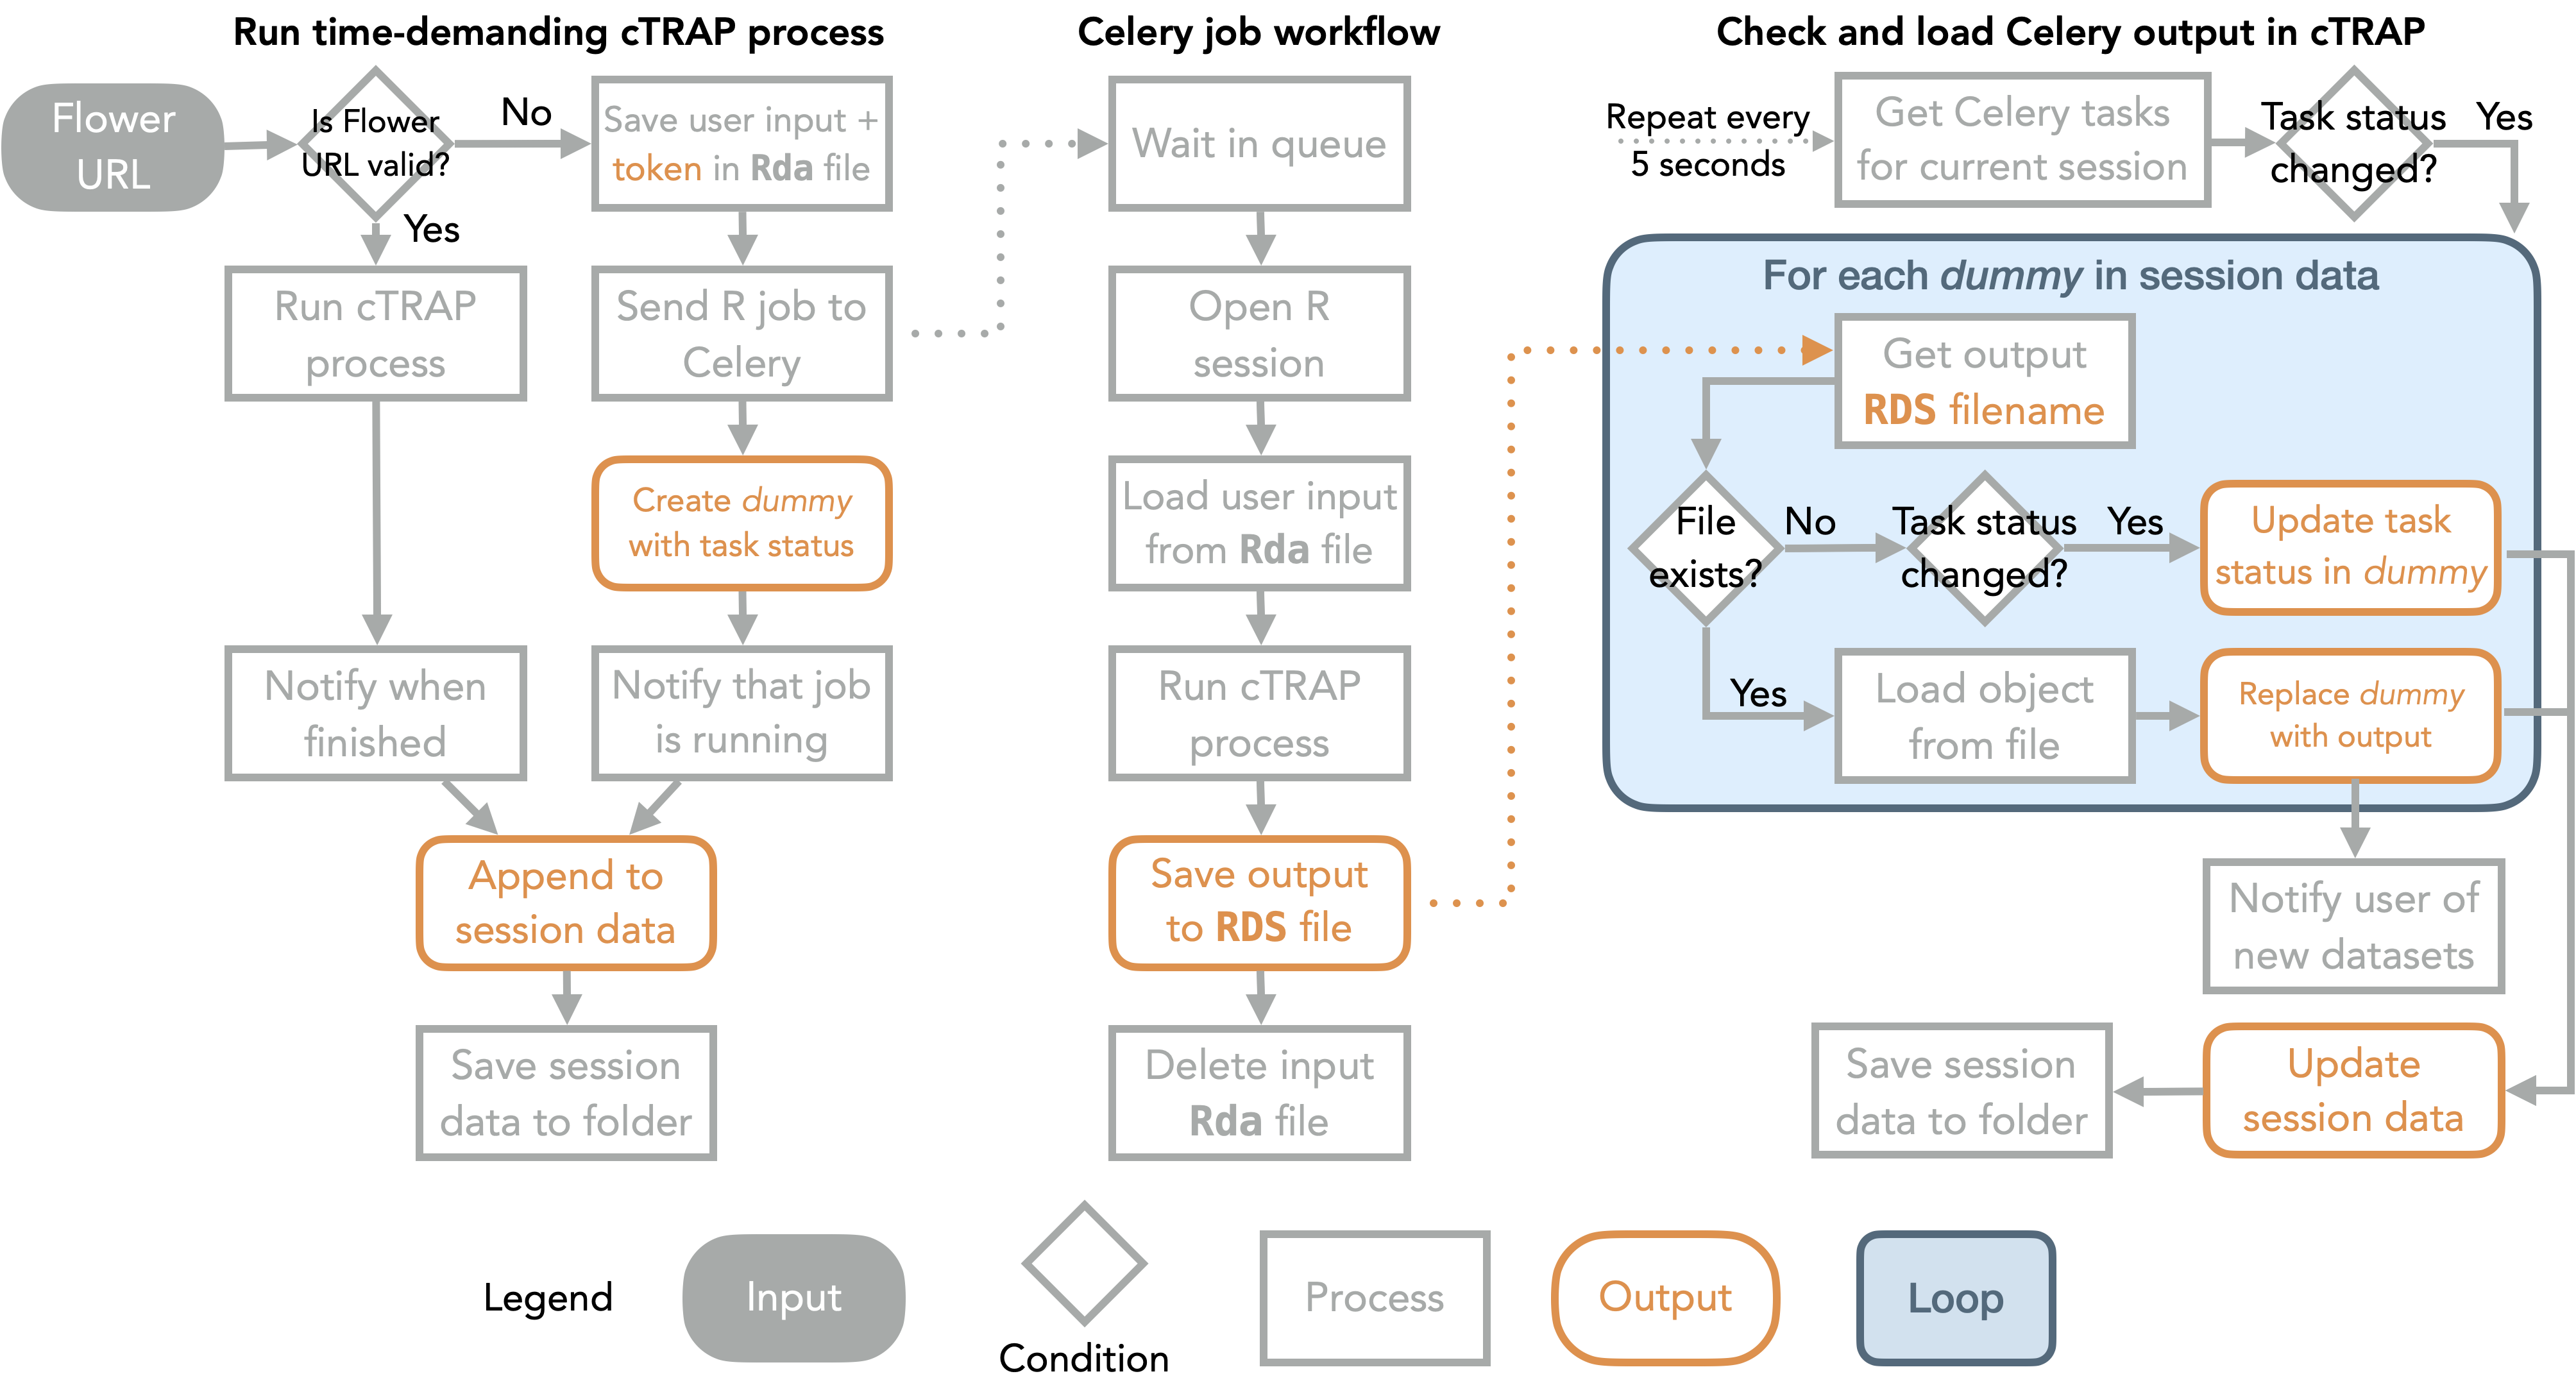
\includegraphics[width=\textwidth]{images/ctrap/celery-job}
  \centering
  \caption[cTRAP process running in Celery]{\textbf{cTRAP process running in Celery.} Time-demanding cTRAP processes can be run in the background using Celery/Flower. While running in Celery, the output of the cTRAP process is saved to the folder associated with the token of the user's session. When that specific session is active, all finished files are automatically loaded as part of the data session and the user is notified.}
  \label{fig:ctrap-celery}
\end{figure}

Why saving \emph{dummy} objects as part of user session data?

\section{Conclusion}

It would also be interesting to send automatic emails to users when a job finishes or raises an error. This would require to set up an email address to which to send emails from.

For future cTRAP iterations, it would interesting to support CMap LINCS 2020, an expansion of the current CMap dataset that is described as a "3-fold expansion on the previous resource, and notable new subsets of data include CRISPSR knockout of \textgreater 5k genes and hematopoietic and non-cancer cell models" (\alink{clue.io/data/CMap2020\#LINCS2020}).

Also, newever versions of drug sensitivity datasets: GDSC 8?
